\documentclass[a4paper, 12pt]{article}%тип документа

%отступы
\usepackage[left=2cm,right=2cm,top=2cm,bottom=3cm,bindingoffset=0cm]{geometry}

%Русский язык
\usepackage[T2A]{fontenc} %кодировка
\usepackage[utf8]{inputenc} %кодировка исходного кода
\usepackage[english,russian]{babel} %локализация и переносы

%Вставка картинок
\usepackage{wrapfig}
\usepackage{graphicx}
\graphicspath{{pictures/}}
\DeclareGraphicsExtensions{.pdf,.png,.jpg}

%оглавление
\usepackage{titlesec}
\titlespacing{\chapter}{0pt}{-30pt}{12pt}
\titlespacing{\section}{\parindent}{5mm}{5mm}
\titlespacing{\subsection}{\parindent}{5mm}{5mm}
\usepackage{setspace}

%Графики
\usepackage{multirow}
\usepackage{pgfplots}
\pgfplotsset{compat=1.9}

%Математика
\usepackage{amsmath, amsfonts, amssymb, amsthm, mathtools}

%Стиль страницы
\usepackage{fancyhdr}
\pagestyle{fancy}

\begin{document}

\begin{titlepage}

\begin{center}
%\vspace*{1cm}
\large\textbf{Московский Физико-Технический Институт}\\
\large\textbf{(национальный исследовательский университет)}
\vfill
\line(1,0){430}\\[3mm]
\huge\textbf{Лабораторная работа №4.2.1}\\
\line(1,0){430}\\[1mm]
\vfill
\large Баканова К.В., Б01-003\\
%\vspace*{1cm}
\large апрель 2022 г.\\
\end{center}

\end{titlepage}
\fancyhead[L] {Лабораторная работа №4.2.1}
\noindent \textbf{Цель работы:} \\
\indent познакомиться с явлением интерференции в тонких плёнках (полосы равной толщины) на примере колец Ньютона и с методикой интерференционных измерений кривизны стеклянной поверхности.\\
\noindent \textbf{В работе используются:} \\
\indent измерительный микроскоп с опак-иллюминатором, плоско-выпуклая линза; пластинка из чёрного стекла, ртутная лампа типа ДРШ, щель, линзы, призма прямого зрения, объектная шкала.
	
\item      	
\item      

\section{Теория}

\fancyhead[L] {Лабораторная работа №4.2.1}
\fancyhead[R] {Баканова К.В.}

\begin{wrapfigure}{l}{0.5\textwidth}
\begin{center}
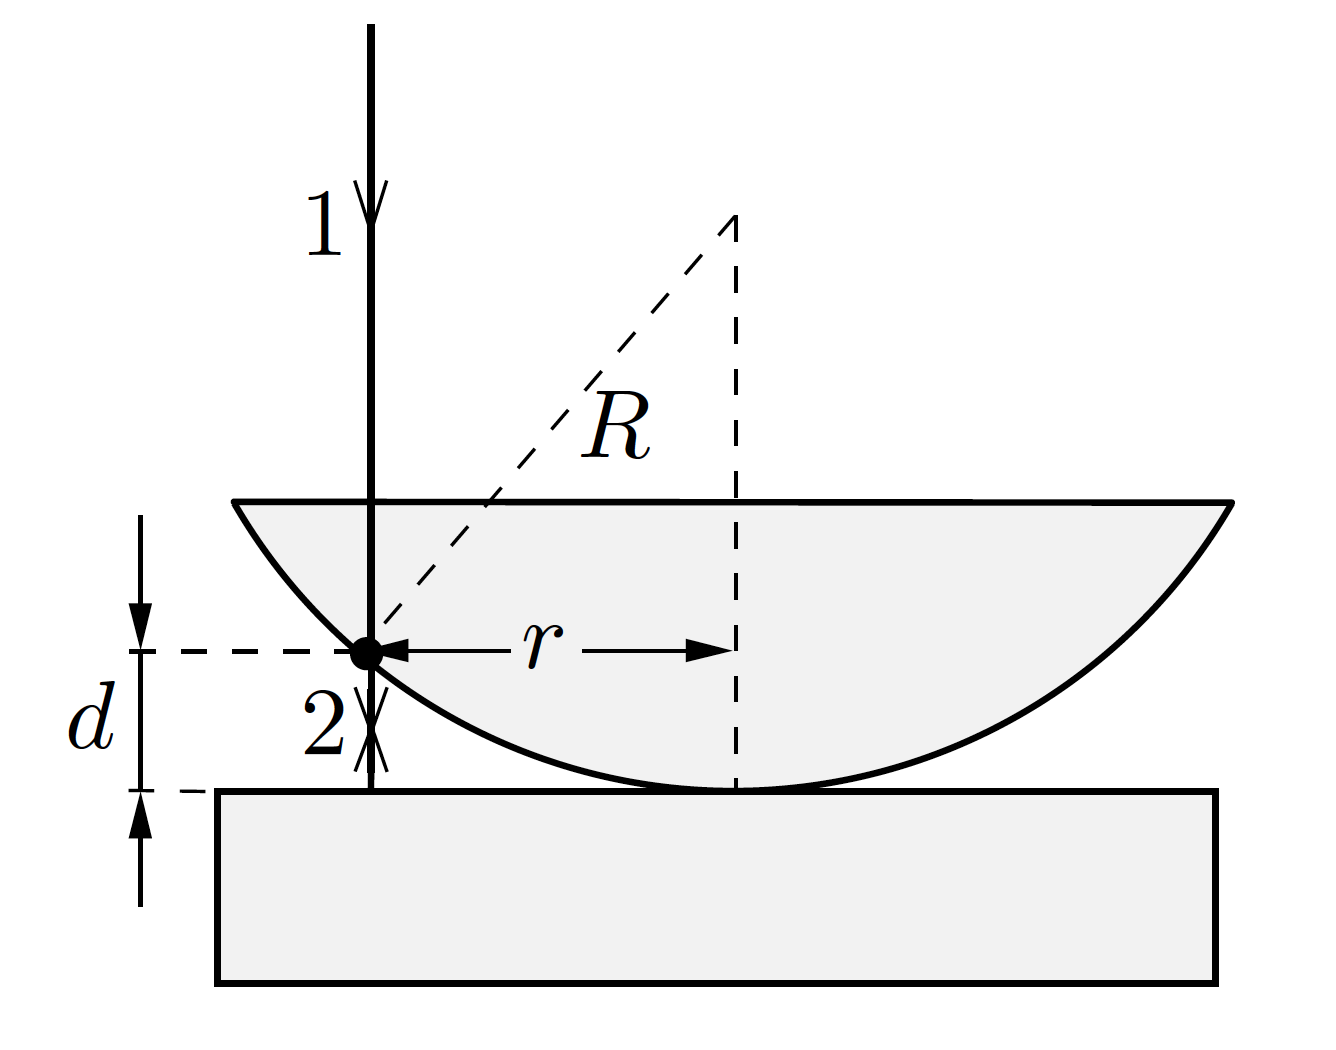
\includegraphics[width = 0.4\textwidth]{ring.png}
\vspace{-20pt}
\end{center}
\caption{Экспериментальная установка}
\end{wrapfigure}

\item Этот классический опыт используется для определения радиуса кривизны сферических поверхностей линз. В этом опыте наблюдается интерференция волн, отражённых от границ тонкой воздушной прослойки, образованной сферической поверхностью линзы и плоской стеклянной пластиной. При нормальном падении света (рис. 1) интерференционные полосы локализованы на сферической поверхности и являются полосами равной толщины.

\item Геометрическая разность хода между интерферирующими лучами равна удвоенной толщине воздушного зазора $ 2d $ в данном месте. Для точки на сферической поверхности, находящейся на расстоянии $ r $ от оси системы, имеем $ r^2 = R^2 - (R - d)^2 = 2Rd - d^2 $, где $ R $ --- радиус кривизны сферической поверхности (рис. 1).

\item При $ R \gg d $ получим $  d = r^2/2R $. С учётом изменения фазы на $ \pi $ при отражении волны от оптически более плотной среды (на границе воздух-стекло) получим \textbf{оптическую разность хода интерферирующих лучей}:

\[\Delta = \dfrac{\lambda}{2} + 2d = \dfrac{r^2}{2R} + \dfrac{\lambda}{2}\]    	
\item      	 
	
\item Из условия интерференционного минимума $ \Delta = \dfrac{(2m +1)\lambda}{2}, \; m =0, 1, 2.. $ получим радиусы темных колец $ r_m $, а из аналогичного условия максимума $ \Delta = m \lambda $ радиусы светлых $ r_m' $ :
	
\item      
\[r_m = \sqrt{m \lambda R}, \qquad 	r_m' = \sqrt{\dfrac{(2m-1)m \lambda R}{2}}\]  

\newpage
	\section{Экспериментальная установка}
\item Схема экспериментальной установки приведена на рис. \ref{lab}. Опыт выполняется с помощью измерительного микроскопа.
На столик микроскопа помещается держатель с полированной пластинкой из
чёрного стекла. На пластинке лежит исследуемая линза.

	\begin{wrapfigure}{r}{0.63\linewidth} 
	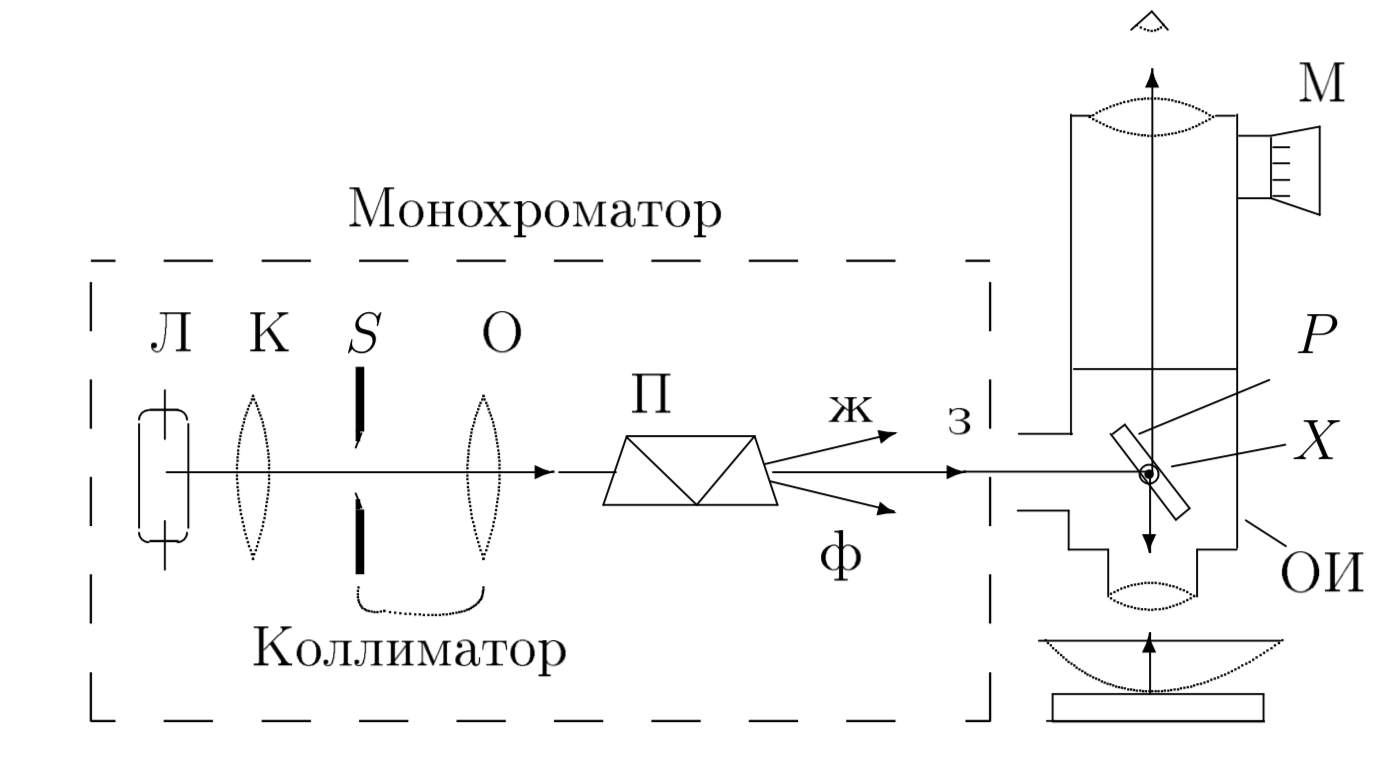
\includegraphics[width=\linewidth]{lab}
	\caption{Экспериментальная установка}
	\label{lab}
\end{wrapfigure}


\item Источником света служит ртутная лампа, находящаяся в защитном кожухе. Для получения монохроматического света применяется призменный монохроматор, состоящий из конденсора $ К $, коллиматора (щель $ S $ и объектив $ О $) и призмы прямого зрения $ П $. Эти устройства с помощью рейтеров располагаются на оптической скамье. Свет от монохроматора попадает на расположенный между объективом и окуляром микроскопа опак-иллюминатор (ОИ)  специальное устройство, служащее для освещения объекта при работе в отражённом свете. Внутри опак-иллюминатора находится полупрозрачная стеклянная пластинка P, наклоненная под углом $ 45^\circ $ к оптической оси микроскопа. Свет частично отражается от этой пластинки, проходит через объектив микроскопа и попадает на исследуемый объект. Пластинка может поворачиваться вокруг горизонтальной оси $ X $, опак-иллюминатор вокруг вертикальной оси.

\item Столик микроскопа может перемещаться в двух взаимно перпендикулярных направлениях помощью винтов препаратоводителя. Отсчетный крест окулярной шкалы перемещается перпендикулярно оптической оси с помощью микрометрического винта $ М $.
	
\item Оптическая схема монохроматора позволяет получить в плоскости входного окна опак-иллюминатора достаточно хорошо разделённые линии спектра ртутной лампы. Изображение щели $ S $ фокусируется на поверхность линзы объективом микроскопа, т.е. точка источника и точка наблюдения спектра совпадают.Интерференционная картина не зависит от показателя преломления линзы и определяется величиной зазора между линзой и пластинкой (кольца равной толщины).

\item Сначала микроскоп настраивается на кольца Ньютона в белом свете (свете ртутной лампы), затем при помощи монохроматора выделить из спектра яркую зелёную линию и провести измерения диаметров колец в монохроматическом свете. 

\item      
	\section{Ход работы}
	
\fancyhead[L] {Лабораторная работа №4.2.1}
\fancyhead[R] {Баканова К.В.}

\item После настройки микроскопа проведем измерения диаметров колец Ньютона. Измерения будем проводить в безразмерных единицах окулярной шкалы, переведённых затем в реальную величину с помощью калиброванной объектной шкалы. 
	
\item Теперь определим калибровку окулярной шкалы. Она равна $ k = 0,1 $ мм.

\item Оценим систематическую погрешность измерения величин на окуляре как $ \sigma_l = 0,02 $ (из-за цены деления).
	
\item C помощью призмы разобьем свет ртутной лампы на зеленый ($ \lambda_g $ = 546 нм) и желтый ($ \lambda_y $ = 578 нм).
	
\item Будем последовательно измерять расстояния $ l_1 $ от верхнего края 7-ого "<набора"> колец до нуля до центра, затем аналогично будем измерять расстояния $ l_2 $ от нижнего края до нуля. Результаты занесем в таблицу. 

\item Построим график зависимости радиусов колец от их номера. 

		\begin{table}[h!]
		\caption{Измерение диаметров колец Ньютона}
		\begin{center}
			\begin{tabular}{|c|c|c|c|c|c|c|}
				\hline
				m & \multicolumn{3}{|c|}{Темные кольца} & \multicolumn{3}{|c|}{Светлые кольца} \\
				\cline{2-7}
				& $ l_1 $& $ l_2 $ & $ r_m^2 $ &$ l_1 $& $ l_2 $ & $ (r_m')^2 $ \\
				\hline
				0 & 4.71 & 3.72 & 0.25 & 4.15 & 4.15 & 0 \\
				1 & 5 & 3.24 & 0.77 & 4.78 & 3.43 & 0.46 \\
				2 & 5.45 & 2.92 & 1.6 & 5.16 & 3.08 & 1.08 \\
				3 & 5.59 & 2.65 & 2.16 & 5.44 & 2.79 & 1.76 \\
				4 & 5.83 & 2.42 & 2.91 & 5.7 & 2.54 & 2.5 \\
				5 & 6.02 & 2.23 & 3.59 & 5.91 & 2.32 & 3.22 \\
				6 & 6.17 & 2.06 & 4.22 & 6.09 & 2.11 & 3.96 \\
				7 & 6.47 & 1.89 & 5.24 & 6.25 & 1.97 & 4.58 \\
				\hline
			\end{tabular}
		\end{center}
		\label{table}
	\end{table}

\begin{figure}[h]
\begin{center}
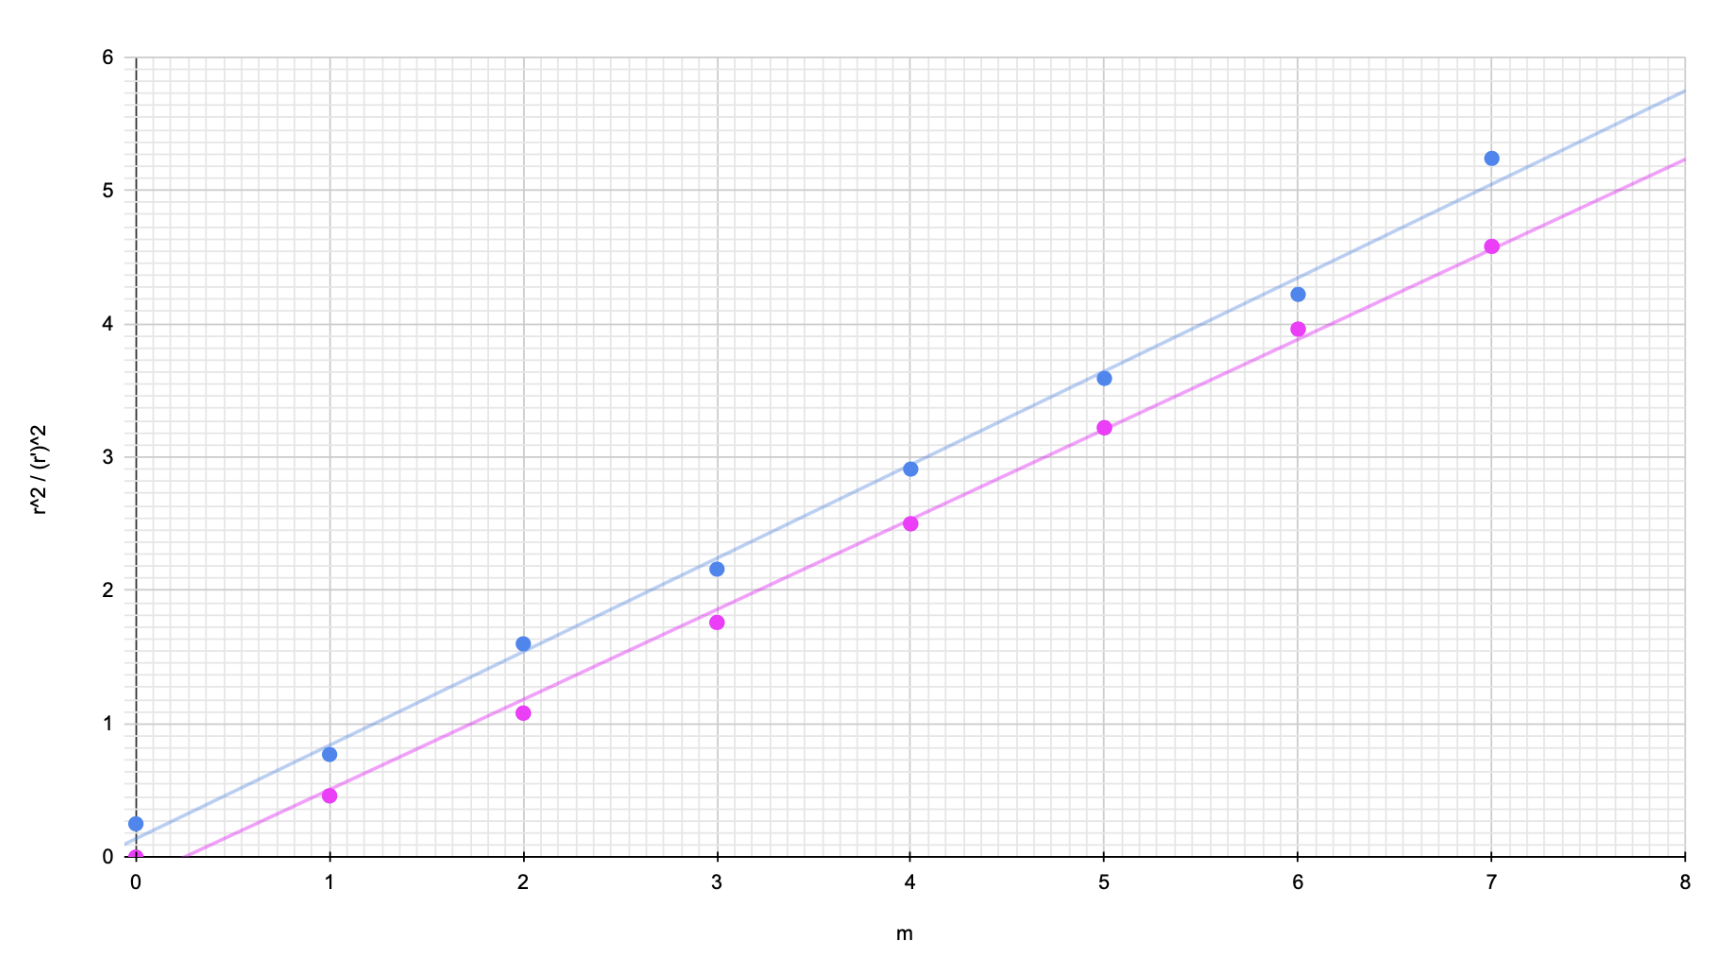
\includegraphics[width = 1.0\textwidth]{graf.png}
\caption{График зависимости $ r_m^2$ и $ (r_m')^2 $ от номера $ m $}
\end{center}
\end{figure}

	\begin{table}[h!]
		\caption{Расчет апроксимированной прямой $ y = ax +b $ для темных колец}
		\begin{center}
		\begin{tabular}{l|ll}
				\text{} & \text{Оценка} & Стандартное отклонение  \\
				\hline
				$ b $ & 0.13 & 0.08  \\
				$ a $ & 0.70 & 0.01  \\
			\end{tabular}
			\end{center}
	\end{table}

	\begin{table}[h!]
		\caption{Расчет апроксимированной прямой $ y = ax +b $ для светлых колец}
		\begin{center}
		\begin{tabular}{l|ll}
			\text{} & \text{Оценка} & Стандартное отклонение  \\
			\hline
			$ b $ & -0.17 & 0.06 \\
	$ 	a $ & 0.67 & 0.01
		\end{tabular}
		\end{center}
	\end{table}

\item При биениях мы наблюдали следующее количество полос между центрами четких систем $ \Delta m =  12 $. Вычислим отсюда разность длин волн желтого и зеленого света ртутной лампы $ \Delta \lambda = \lambda_y - \lambda_g $:

\[(\Delta m + 1)\lambda_g = \Delta m \lambda_y \rightarrow \Delta \lambda = \dfrac{\lambda_g}{\Delta m} \approx \fbox{45 \: \text{нм} }\]

\item Далее вычислим цену деления окулярной шкалы. На 5.67 ед. шкалы помещается 60 делений (0.6 мм), т.е.:
\[\dfrac{0,6}{5,67} = 0,106 \dfrac{\: \text{мм}}{\: \text{ед. шкалы}}\]

\item Определим радиус кольца. Так как $ \dfrac{r^2_m}{m} = k^2 \x a_т$, отсюда

\item         
\[R = \dfrac{r^2_m}{m \lambda} = \fbox{(1,28 \pm 0,02) \: \text{cм} }\]

\item         

	\section{Вывод}
	
\item Мы получили из эксперимента, что разница длин волн желтого и зеленого света ртутной лампы примерно равна $  \Delta \lambda = 45 \: \text{нм}$, в то время как табличный результат = 33 нм. Это возникает вследствие большой неточности определения числа $ \Delta m $. Также по графикам зависимости радиусов колец Ньютона от их номеров нам удалось рассчитать радиус линзы ---  $ R = (1,28 \pm 0,02) \: \text{cм} $.


	
\end{document}



